\appendix  \label{app}
\addappheadtotoc 
\appendixpage

En este ap\'endice se incorporan todos los elementos del sistema digestivo, expuestos por el/los autores de los diferentes materiales en los cuales, 
pero no limitados a estos, se realizó la investigación del sistema, cabe mencionar que en algunas figuras que se muestran se incluyen elementos 
que no son parte de los componentes del sistema digestivo pero estos se incluyen en las figuras debido a que son parte de la cavidad abdominal, 
o en su defecto el órgano en el cual se está centrando el desarrollo del modelo se encuentra demasiado cerca de un órgano u órganos contiguos 
para ser incluido en la figura individualmente.\\

\section{Glándulas salivales}
Las glándulas salivales son glándulas exocrinas (glándulas con un conducto excretor por el que sale la sustancia que elaboran) del complejo digestivo 
superior. Estas segregan saliva. El sistema de  glándulas salivales se diferencian o clasifican por  su tamaño y por la función que realizan dentro 
del cuerpo humano, dividiéndose en dos grupos.\\ 
Dos parótidas: con unas dimensiones de 6 cm de longitud y 3-4 de ancho cada una, son las glándulas de mayor tamaño, están dispuestas bilateralmente 
(a ambos lados de la cara) justo detrás del ángulo de la mandíbula, por debajo y delante de los oídos. Son las que producen más cantidad de saliva.
Dos submandibulares: se sitúan en el suelo de la boca. Son las más pequeñas de las glándulas mayores. Se encuentran envueltas de tejido conjuntivo.
Dos sublinguales: situadas a una profundidad mayor en el suelo de la cavidad oral a posterior. Llamadas también glándulas submandibulares. Su forma 
es irregular y de un tamaño aproximado al de una nuez.\\
\begin{figure}[H]
	\begin{center}
 		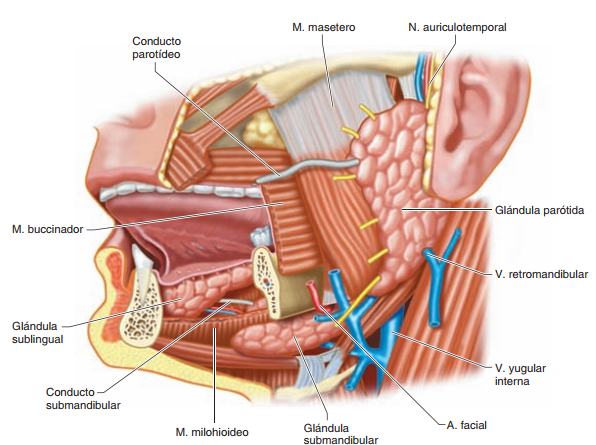
\includegraphics[width = .7\textwidth]{v2/images/image34.png}
 		\captionof{figure}{\label{fig:a1}Glándula parótida}
	\end{center} 
\end{figure}

\section{Cavidad Oral y Faringe}
Los modelos de la cavidad oral se mostrarán en conjunto con los de la faringe dado que son parte de un mismo conjunto.\\
Las mejillas y los labios limitan la cavidad oral, con un espacio (el vestíbulo) entre las mejillas, los labios y los dientes. Las mejillas contienen 
el músculo buccinador que, junto con la lengua, mantiene el alimento entre los dientes durante la masticación.\\
La faringe se sitúa por detrás y por debajo de la boca. Cuando los alimentos y líquidos salen de la boca, descienden a través de la garganta. 
La deglución de los alimentos y de los líquidos comienza de manera voluntaria y continúa de forma automática. Una pequeña lengüeta muscular (epiglotis) 
se cierra para evitar que los líquidos y los alimentos bajen por la tráquea hacia los pulmones. El velo del paladar se eleva para evitar que suban a la nariz. 
La úvula, una pequeña solapa unida al velo del paladar, ayuda a evitar que asciendan los líquidos hacia el interior de la cavidad nasal.\\
\begin{figure}[H]
	\begin{center}
 		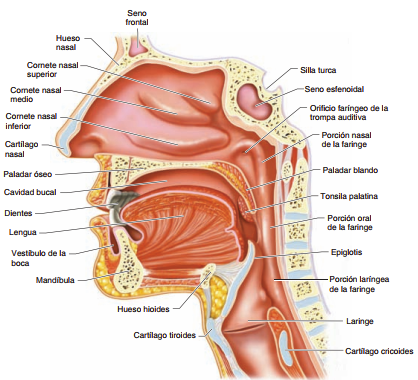
\includegraphics[width = .7\textwidth]{v2/images/image84.png}
 		\captionof{figure}{\label{fig:a2}Cavidad bucal (corte sagital)}
	\end{center} 
\end{figure}
\begin{figure}[H]
	\begin{center}
 		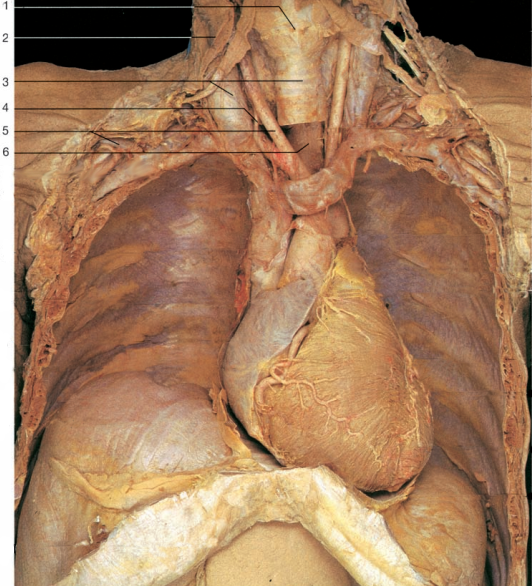
\includegraphics[width = .7\textwidth]{v2/images/image42.png}
 		\captionof{figure}{\label{fig:a3}Corazón y vasos relacionados in situ (aspecto anterior). Se han eliminado la pared
         torácica anterior, el pericardio y el epicardio, se ha dividido la tráquea}
	\end{center} 
\end{figure}
\begin{enumerate}
    \item Laringe (cartílago tiroideo)
    \item Músculo esternocleidomastoideo (dividido)
    \item Tráquea (dividida) y vena yugular interna derecha
    \item Nervio vago
    \item Derecha arteria carótida común y vena cefálica
    \item Esófago    
\end{enumerate}

\section{Esófago}
El esófago es un canal muscular de paredes finas, recubierto en su interior por membranas mucosas, que conecta la garganta con el estómago. Los alimentos 
y líquidos son propulsados a través del esófago no solo por la gravedad sino también por ondas de contracciones musculares rítmicas, lo que se denomina peristaltismo. 
En ambos extremos del esófago existen dos músculos en forma de anillo (esfínteres esofágicos superior e inferior), que se abren y cierran. Normalmente, los esfínteres 
esofágicos impiden que el contenido del estómago vuelva a pasar al esófago o a la garganta.\\
El esófago forma parte de su tubo digestivo. Es el \"conducto alimentario\" que conecta su garganta con su estómago. Los alimentos y los líquidos no solo descienden por 
el esófago a causa de la gravedad. Su esófago está revestido de músculos que empujan los alimentos y los líquidos hacia abajo.\\
Otros músculos rodean los extremos superior e inferior de su esófago como si fueran anillos. Estos músculos, también llamados esfínteres, cierran el esófago para que 
el contenido de su estómago no pueda regresar al esófago o a la garganta.\\
\begin{figure}[H]
	\begin{center}
 		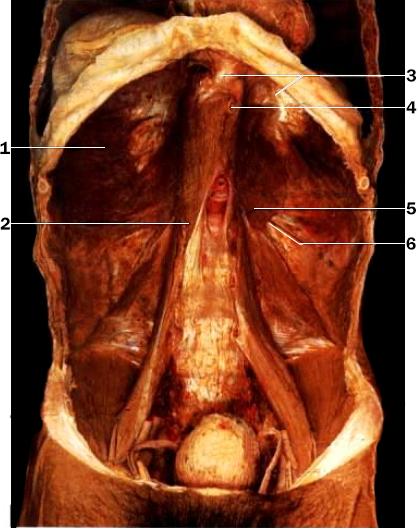
\includegraphics[width = .7\textwidth]{v2/images/image39.png}
 		\captionof{figure}{\label{fig:a4}Diafragma y pared abdominal (vista anterior)}
	\end{center} 
\end{figure}
\begin{enumerate}
    \item Diafragma porción costal
    \item Arco costal
    \item Diafragma centro frénico
    \item Esófago
    \item Diafragma arco del psoas
    \item Diafragma cuadrado lumbar    
\end{enumerate}

\section{Estómago}
El estómago es un órgano muscular grande, hueco y con forma de alubia, en el que se distinguen tres regiones o zonas:\\
\begin{itemize}
    \item Cardias
    \item Cuerpo (fondo)
    \item Antro pilórico    
\end{itemize}
Los alimentos y los líquidos llegan al estómago desde el esófago pasando a través del esfínter esofágico inferior.\\
La parte superior del estómago sirve como área de almacenamiento para los alimentos. Aquí, el cardias y el cuerpo gástrico (fondo) se relajan para acomodar el alimento 
que entra en el estómago. A continuación el antro pilórico (la parte inferior del estómago) se contrae rítmicamente, mezclando el alimento con ácido y enzimas (jugos gástricos) 
y triturando en pequeños fragmentos para facilitar su digestión. Las células que recubren la superficie gástrica secretan tres sustancias importantes: moco, ácido clorhídrico 
y el precursor de la pepsina (una enzima que fracciona las proteínas). El moco recubre las células de la superficie gástrica para protegerlas de lesiones causadas por el ácido 
y las enzimas.\\
El ácido clorhídrico proporciona un ambiente sumamente ácido, necesario para que la pepsina descompone las proteínas. La elevada acidez del estómago también actúa como una barrera 
contra las infecciones, pues elimina la mayor parte de las bacterias. La secreción ácida es estimulada por impulsos nerviosos que llegan al estómago, por la gastrina (una hormona 
que secreta el estómago) y por la histamina (otra sustancia liberada en el estómago). La pepsina es la única enzima que digiere el colágeno, una proteína que es, a su vez, parte 
importante de la carne.\\
\begin{figure}[H]
	\begin{center}
 		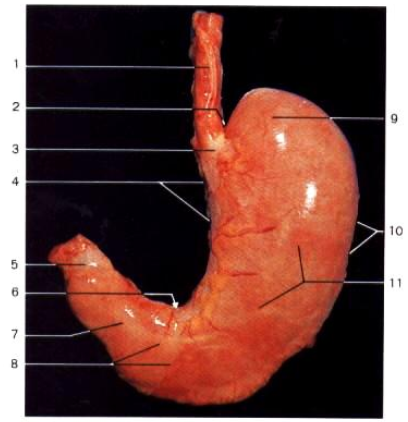
\includegraphics[width = .7\textwidth]{v2/images/image2.png}
 		\captionof{figure}{\label{fig:a5}Vista anterior del estómago y sus relaciones}
	\end{center} 
\end{figure}
\begin{enumerate}
    \item Esófago
    \item Escotadura cardiaca
    \item Porción cardiaca del estómago
    \item Curvatura menor del estómago
    \item Esfínter pilórico
    \item Escotadura angular
    \item Antro pilórico
    \item Porción pilórica del estómago
    \item Fondo del estómago
    \item Curvatura mayor del estómago 
    \item Cuerpo del estómago    
\end{enumerate}

\section{Intestino delgado}
El duodeno es el primer segmento del intestino delgado, y el estómago vierte el alimento en su interior. El alimento entra en el duodeno a través del esfínter pilórico en 
cantidades que el intestino delgado pueda digerir. Cuando se llena, el duodeno envía una señal al estómago para detener la evacuación.\\
El duodeno recibe enzimas pancreáticas del páncreas, y bilis del hígado y de la vesícula biliar. Estos fluidos, que llegan al duodeno a través de una abertura denominada 
esfínter de Oddi, contribuyen de modo importante en la digestión y la absorción. Las ondas de contracciones musculares rítmicas (denominadas peristaltismo) también contribuyen 
a la digestión y a la absorción removiendo los alimentos y mezclandolos con las secreciones.\\
Los centímetros iniciales del revestimiento duodenal son lisos, pero el resto presenta pliegues, pequeños salientes (vellosidades) e incluso salientes aún más pequeños 
(microvellosidades). Estas vellosidades y microvellosidades incrementan el área de la superficie de revestimiento del duodeno, permitiendo así una mayor absorción de nutrientes.\\
El resto del intestino delgado está formado por el yeyuno y el íleon, que están situados por debajo del duodeno. Estas partes del intestino delgado son en gran medida responsables 
de la absorción de grasas y otros nutrientes. Los movimientos de batido facilitan la absorción. La absorción también se incrementa debido a la extensa superficie formada por los 
pliegues, vellosidades y microvellosidades. La pared intestinal está muy irrigada por vasos sanguíneos que conducen los nutrientes absorbidos hacia el hígado a través de la vena 
porta. La pared intestinal libera moco que lubrica el contenido intestinal y agua que ayuda a disolver los fragmentos digeridos. También se liberan pequeñas cantidades de enzimas 
que digieren las proteínas, los azúcares y las grasas.\\
La consistencia del contenido intestinal cambia gradualmente a medida que este avanza por el intestino delgado. En el duodeno, el alimento es diluido con enzimas pancreáticas 
y bilis, que disminuyen la acidez estomacal. El contenido continúa su paso por el intestino delgado, haciéndose más líquido a medida que se mezcla con agua, moco, bilis y enzimas 
pancreáticas. Finalmente, el intestino delgado absorbe la mayor parte de los nutrientes y casi todo el líquido (a excepción de aproximadamente un litro) antes de pasarlo al intestino 
grueso. [ 50 ]\\
\begin{figure}[H]
	\begin{center}
 		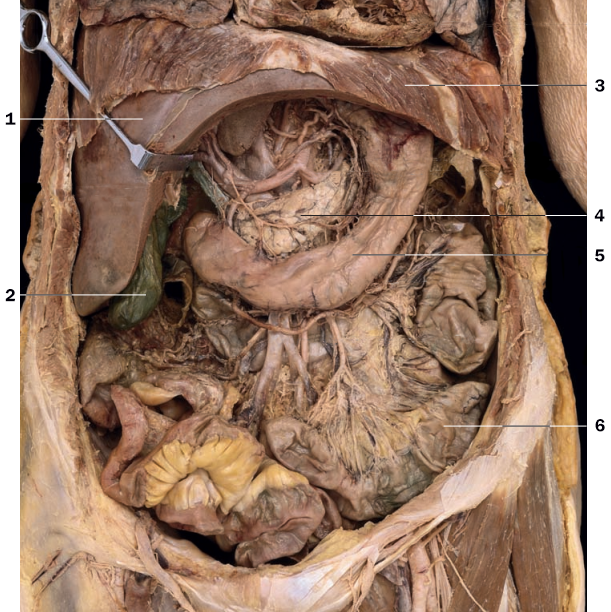
\includegraphics[width = .7\textwidth]{v2/images/image79.png}
 		\captionof{figure}{\label{fig:a6}Vasos de los órganos abdominales superiores y del intestino delgado (aspecto anterior). Disección de la vena mesentérica superior. El hígado está disecado y elevado. [ 51 ]}
	\end{center} 
\end{figure}
\begin{itemize}
    \item Hígado
    \item Vesícula biliar
    \item Diafragma
    \item Páncreas
    \item Estómago
    \item Intestino Delgado    
\end{itemize}

\section{Hígado}
El hígado, con forma de cuña, es el órgano más grande y, en algunos aspectos, el más complejo del cuerpo humano. Sirve como la fábrica de productos químicos del organismo, desempeñando 
muchas funciones vitales que incluyen desde la regulación de compuestos químicos en el organismo hasta la producción de sustancias que hacen que la sangre se coagule (factores de coagulación) 
durante una hemorragia. \\
El hígado produce casi la mitad del colesterol del organismo. El resto proviene de los alimentos. La mayor parte del colesterol fabricado en el hígado se utiliza para la producción de bilis, 
un líquido espeso, viscoso y de color amarillo verdoso que ayuda a la digestión. El colesterol también es necesario para sintetizar ciertas hormonas, incluidos los estrógenos, la testosterona 
y las hormonas suprarrenales, y es un componente esencial de todas las membranas celulares. El hígado elabora otras sustancias, entre ellas las proteínas que el organismo necesita para llevar 
a cabo sus funciones. Por ejemplo, los factores de la coagulación son proteínas necesarias para detener los sangrados. La albúmina es una proteína necesaria para mantener la presión de los 
líquidos en el torrente sanguíneo.\\
Los azúcares son almacenados en el hígado en forma de glucógeno y posteriormente descompuestos y liberados al torrente sanguíneo en forma de glucosa a medida que el organismo la necesita, 
como ocurre, por ejemplo, durante el sueño, cuando una persona pasa muchas horas sin comer y los niveles de azúcar en sangre se vuelven demasiado bajos.\\
El hígado también descompone sustancias nocivas o tóxicas (toxinas) absorbidas desde el intestino o producidas en otras partes del organismo, y las excreta luego como subproductos inocuos 
a la bilis o la sangre. Los subproductos excretados a la bilis pasan al intestino y son eliminados del organismo en las heces. Los subproductos excretados a la sangre son filtrados por los 
riñones y posteriormente eliminados del organismo en la orina. El hígado también altera químicamente (metaboliza) los fármacos, con frecuencia activandolos o haciendo más fácil su excreción.\\
El hígado recibe sangre directamente de los intestinos y también del corazón, como lo hacen todos los demás órganos. La sangre de los intestinos contiene casi todo lo absorbido por estos, i
ncluyendo nutrientes, fármacos y a veces toxinas. Esta sangre fluye a través de diminutos capilares de la pared intestinal hacia el interior de la vena porta, que desemboca en el hígado. 
Después la sangre fluye a través de una red de minúsculos canales dentro del hígado, donde se procesan los nutrientes digeridos y las toxinas.\\
La arteria hepática lleva sangre al hígado desde el corazón. Esta sangre transporta oxígeno hacia los tejidos hepáticos, así como colesterol y otras sustancias para ser transformadas. 
La sangre procedente del intestino y la que proviene del corazón se mezclan en los tejidos hepáticos y retornan al corazón por la vena hepática.\\
\begin{figure}[H]
	\begin{center}
 		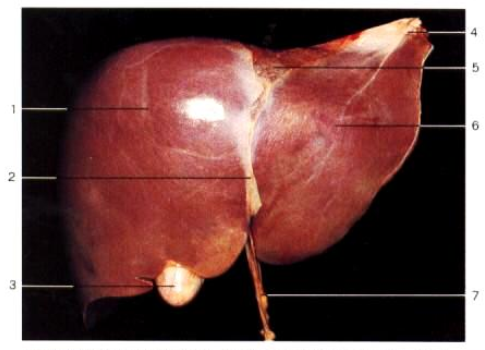
\includegraphics[width = .7\textwidth]{v2/images/image12.png}
 		\captionof{figure}{\label{fig:a7}Vista anterior del hígado}
	\end{center} 
\end{figure}
\begin{enumerate}
    \item Lóbulo derecho
    \item Ligamento falciforme
    \item Vesícula biliar
    \item Ligamento triangular izquierdo
    \item Gran zona desprovista de peritoneo
    \item Lóbulo izquierdo
    \item Ligamento redondo    
\end{enumerate}

\section{Páncreas y vesícula biliar}
El páncreas es un órgano que contiene dos tipos de tejido glandular:\\
\begin{itemize}
    \item Acinos pancreáticos
    \item Islotes de Langerhans    
\end{itemize}
Los ácidos producen enzimas digestivas. Los islotes producen hormonas. El páncreas secreta enzimas digestivas al duodeno y hormonas al torrente sanguíneo.\\
Las enzimas digestivas (como la amilasa, la lipasa y la tripsina) son liberadas por las células de los acinos y circulan por el interior del conducto pancreático. 
El conducto pancreático se une al colédoco en el esfínter de Oddi, por el cual ambos desembocan en el duodeno. Las enzimas son secretadas normalmente en forma inactiva; 
solo se activan cuando alcanzan el tubo digestivo. La amilasa digiere los carbohidratos, la lipasa digiere las grasas y la tripsina digiere las proteínas. El páncreas 
también secreta grandes cantidades de bicarbonato sódico, que protege el duodeno porque ejerce una acción neutralizadora sobre el ácido procedente del estómago.\\
Las tres hormonas producidas por el páncreas son:\\
\begin{enumerate}
    \item Insulina
    \item Glucagón
    \item Somatostatina    
\end{enumerate}
La insulina disminuye el nivel de azúcar (glucosa) en sangre, ya que transporta el azúcar hacia el interior de las células. El glucagón aumenta el nivel de azúcar (glucosa) 
en sangre mediante la estimulación del hígado para que libere sus reservas. La somatostatina evita la liberación de las otras dos hormonas.\\
La vesícula biliar es un pequeño saco muscular de almacenamiento, en forma de pera, que contiene la bilis y que está interconectado con el hígado mediante unos conductos 
llamados vías biliares.\\
La bilis es un líquido espeso y viscoso, de color amarillo verdoso. Se compone de sales biliares, electrolitos (partículas cargadas disueltas, como el sodio y el bicarbonato), 
pigmentos biliares, colesterol y otras grasas (lípidos). La bilis tiene dos funciones principales:\\
\begin{itemize}
    \item Ayudar a la digestión
    \item Eliminar del organismo ciertos productos de desecho (principalmente hemoglobina y exceso de colesterol).    
\end{itemize}
Las sales biliares contribuyen a la digestión haciendo que el colesterol, las grasas y las vitaminas liposolubles sean más fáciles de absorber por el intestino.\\
La bilirrubina es el principal pigmento de la bilis. La bilirrubina es un producto de desecho que se forma a partir de la hemoglobina (la proteína que transporta 
oxígeno en la sangre) y que es excretado en la bilis. La hemoglobina se libera cuando se destruyen los glóbulos rojos (eritrocitos) viejos o dañados.\\
La bilis sale del hígado por los conductos hepáticos derecho e izquierdo, los cuales se unen para formar el conducto hepático común. Posteriormente, este conducto 
se une a otro que está conectado con la vesícula biliar, denominado conducto cístico, para formar el colédoco. Este desemboca en el intestino delgado a través del 
esfínter de Oddi (un músculo en forma de anillo), situado unos centímetros por debajo del estómago.\\
Aproximadamente la mitad de la bilis secretada entre las comidas fluye directamente a través del colédoco al intestino delgado. La bilis restante es desviada a 
través del conducto cístico a la vesícula biliar, donde es almacenada. En la vesícula biliar, hasta el 90\% del agua de la bilis se absorbe hacia el torrente sanguíneo, 
por lo que la bilis restante se vuelve muy concentrada.\\
Cuando entran alimentos en el intestino delgado, una serie de señales hormonales y nerviosas desencadenan la contracción de la vesícula biliar, y la relajación y la apertura del 
esfínter de Oddi. La bilis fluye entonces desde la vesícula biliar hasta el intestino delgado, donde se mezcla con el contenido alimenticio y lleva a cabo sus funciones digestiva\\
\begin{figure}[H]
	\begin{center}
 		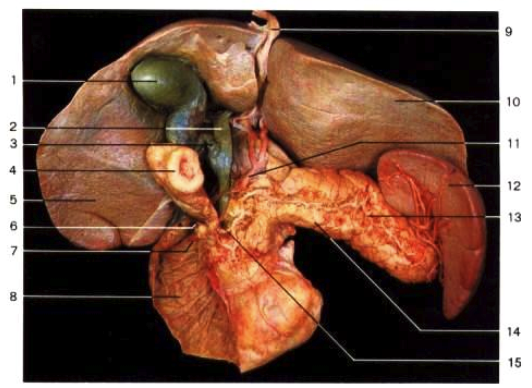
\includegraphics[width = .7\textwidth]{v2/images/image20.png}
 		\captionof{figure}{\label{fig:a8} Páncreas y duodeno, bazo, vesícula biliar e hígado (vista anterior).}
	\end{center} 
\end{figure}
\begin{enumerate}
    \item Vesícula biliar
    \item Conducto hepático común
    \item Conducto cístico
    \item Píloro (seccionado)
    \item Lóbulo derecho del hígado
    \item Carúncula duodenal menor (marcador)
    \item Carúncula duodenal mayor (marcador)
    \item Duodeno
    \item Ligamento redondo del hígado
    \item Lóbulo izquierdo del hígado
    \item Arteria hepática
    \item Bazo
    \item Conducto pancreático de Winsung
    \item Páncreas
    \item Conducto pancreático accesorio de Santorini    
\end{enumerate}
\begin{figure}[H]
	\begin{center}
 		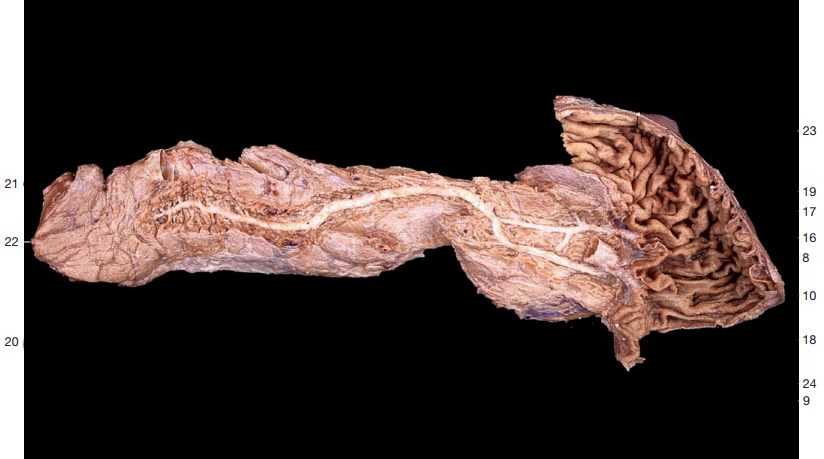
\includegraphics[width = .7\textwidth]{v2/images/image7.png}
 		\captionof{figure}{\label{fig:a9}Páncreas con parte descendente del duodeno (aspecto posterior). El duodeno se abrió para mostrar las papilas duodenales. El conducto pancreático ha sido disecado, el conducto biliar común ha sido dividido}
	\end{center} 
\end{figure}
\section{Intestino grueso y ano}
Las partes del intestino grueso son:\\
\begin{itemize}
    \item Ciego y colon ascendente (derecho)
    \begin{itemize}
        \item Colon transverso
        \item Colon descendente (izquierdo)
        \item Colon sigmoide (que está conectado al recto)
    \end{itemize}
\end{itemize}
El ciego, que se encuentra al principio del colon ascendente, es el punto donde el intestino delgado se une con el intestino grueso. Desde el ciego se proyecta el apéndice, 
una estructura tubular en forma de dedo que no cumple ninguna función conocida. El intestino grueso secreta moco y es responsable en gran medida de la absorción del agua de las heces.\\
El contenido intestinal es líquido cuando llega al intestino grueso, pero normalmente se solidifica durante el tiempo que tarda en alcanzar el recto formando las heces. 
Las numerosas bacterias que habitan en el intestino grueso pueden digerir aún más algunas materias, produciendo gas. Las bacterias del intestino grueso también producen 
algunas sustancias importantes, como la vitamina K, que desempeña un papel relevante en el proceso de coagulación de la sangre. Estas bacterias son necesarias para una 
adecuada función intestinal, y algunas enfermedades y antibióticos pueden alterar el equilibrio entre los diferentes tipos de bacterias que habitan en el intestino grueso.\\
\begin{figure}[H]
	\begin{center}
 		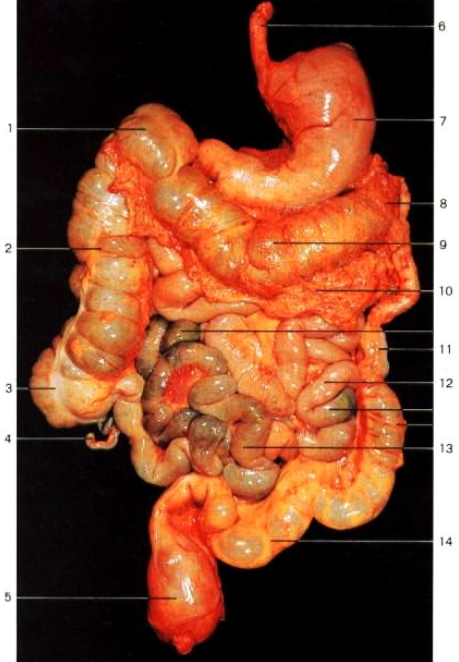
\includegraphics[width = .7\textwidth]{v2/images/image58.png}
 		\captionof{figure}{\label{fig:a10}Tracto gastrointestinal}
	\end{center} 
\end{figure}
\begin{enumerate}
    \item Ángulo hepático del colon
    \item Colon ascendente
    \item Ciego
    \item Apendice veriforme
    \item Recto
    \item Esófago (seccionado)
    \item Estómago
    \item Ángulo esplénico del colon (izquierdo)
    \item Colon transverso
    \item Epiplón mayor
    \item Yeyuno
    \item Íleon
    \item Colon sigmoide
    \item Colon sigmoide    
\end{enumerate}
El ano es la abertura que existe al final del tubo digestivo, por la cual las heces abandonan el organismo. El ano está formado, en parte, por las capas superficiales del cuerpo, 
incluida la piel, y, en parte, por el intestino. Está recubierto por una prolongación de la piel externa. Un anillo muscular, denominado esfínter anal, mantiene el ano cerrado hasta 
que la persona hace una deposición.

%\begin{figure}[H]
%	\begin{center}
% 		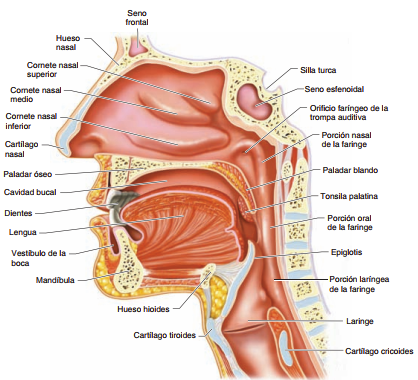
\includegraphics[width = 1\textwidth]{v2/images/image84.png}
% 		\captionof{figure}{\label{fig:a2}Cavidad bucal (corte sagital)}
%	\end{center} 
%\end{figure}